%%%%%%%%%%%%%%%%%%%%%%%%%%%%%%%%%%%%%%%%%%%%%%%%%%%%%%%%%%%%%%%%%%%%%%%%%%%%
% AGUJournalTemplate.tex: this template file is for articles formatted with LaTeX
%
% This file includes commands and instructions
% given in the order necessary to produce a final output that will
% satisfy AGU requirements, including customized APA reference formatting.
%
% You may copy this file and give it your
% article name, and enter your text.
%
%
% Step 1: Set the \documentclass
%
% There are two options for article format:
%
% PLEASE USE THE DRAFT OPTION TO SUBMIT YOUR PAPERS.
% The draft option produces double spaced output.
%

%% To submit your paper:
\documentclass[draft]{agujournal2019}
\usepackage{url} %this package should fix any errors with URLs in refs.
\usepackage{lineno}
\usepackage{color}
\graphicspath{ {figures/} }
\linenumbers
%%%%%%%
% As of 2018 we recommend use of the TrackChanges package to mark revisions.
% The trackchanges package adds five new LaTeX commands:
%
%  \note[editor]{The note}
%  \annote[editor]{Text to annotate}{The note}
%  \add[editor]{Text to add}
%  \remove[editor]{Text to remove}
%  \change[editor]{Text to remove}{Text to add}
%
% complete documentation is here: http://trackchanges.sourceforge.net/
%%%%%%%

\draftfalse

\journalname{JGR: Space Physics}


\begin{document}

\title{Microburst Scale Size Distribution Derived with AeroCube-6}

%% ------------------------------------------------------------------------ %%
%
%  AUTHORS AND AFFILIATIONS
%
%% ------------------------------------------------------------------------ %%

\authors{M. Shumko\affil{1}, J. Sample\affil{1}, A. Johnson\affil{1}, D.L. Turner\affil{2}, T.P. O'Brien\affil{2},  B.A. Griffith\affil{1}, J.B. Blake\affil{2}, O. Agapitov\affil{3}, S. G. Claudepierre\affil{2}}


\affiliation{1}{Department of Physics, Montana State University, Bozeman, Montana, USA}
\affiliation{2}{Space Science Applications Laboratory, The Aerospace Corportation, El Segundo, California, USA}
\affiliation{3}{Space Sciences Laboratory, University of California berkeley, Berkeley, California, USA}

\correspondingauthor{M. Shumko}{msshumko@gmail.com}

\begin{keypoints}
\item The dual AeroCube-6 CubeSats simultaneously observed $> 35$ keV microbursts at a variety of spatial separations ranging from $2$ to $\approx 100$ km.
\item In low Earth orbit the majority of microbursts have a size on the order of a few tens of km.
\item At the magnetic equator the size of most microbursts correlate to the size of correlated whistler-mode chorus waves.
\end{keypoints}

%% ------------------------------------------------------------------------ %%
%
%  ABSTRACT
%
% A good abstract will begin with a short description of the problem
% being addressed, briefly describe the new data or analyses, then
% briefly states the main conclusion(s) and how they are supported and
% uncertainties.
%% ------------------------------------------------------------------------ %%

%% \begin{abstract} starts the second page

\begin{abstract}
Microbursts are an impulsive increase of electrons from the radiation belts into the atmosphere and have been directly observed in low Earth orbit and the upper atmosphere. Microburst are believed to be generated by scattering of radiation belt electrons by whistler mode waves. Prior work has estimated that microbursts are capable of rapidly depleting the radiation belt electrons on the order of a day, hence their role to radiation belt electron losses must be considered. Radiation belt electron losses due to microbursts are not well constrained, and more work is necessary to accurately quantify their contribution as a loss process. To address this question we present a statistical study of $> 30$ keV microburst sizes using the pair of AeroCube-6 CubeSats. The microburst size distribution in low Earth orbit and the magnetic equator was derived. In low Earth orbit, the majority of microbursts were observed while the AC6 separation was less than a few tens of km. Most observed microburst map to sizes less then $200$ km at the magnetic equator which corresponds to highly correlated whistler mode chorus scale size derived in prior literature.
\end{abstract}

\section{Plain Language Summary}
\textcolor{red}{https://sharingscience.agu.org/creating-plain-language-summary/}

\section{Introduction}
Since the discovery of the Van Allen radiation belts in the 1960s by \citeA{Allen1959} and \citeA{Vernov1960}, decades of research has made headway in understanding the various particle acceleration and loss mechanisms. One of the extensively studied mechanisms responsible for both acceleration and loss is wave-particle scattering between whistler-mode chorus waves and electrons \cite{Abel1998_1, Meredith2002, Horne2003, Thorne2005, Millan2007, Bortnik2008}. Whistler-mode chorus waves are typically generated by a temperature anisotropy of low energy electrons up to tens of kiloelectronvolts (keV) and are typically found in the $\sim 0-12$ magnetic local times (MLT) \cite{Li2009, Li2009b}. Whistler-mode chorus waves interact with radiation belt electrons, and are widely believed to cause electron precipitation termed microbursts \cite<e.g.,>[]{Millan2007} 

Microbursts are a subsecond impulse of electrons that are observed by high altitude balloons and satellites in low Earth orbit (LEO) on the radiation belt magnetic footprints, $\sim 4 - 8$ L-shell (L) \cite<e.g.,>[]{Anderson1964, Parks1967, Lorentzen2001a, Lorentzen2001b, O'Brien2003, Woodger2015, Crew2016, Breneman2017, Mozer2018, Greeley2019}. Microburst`s role as a radiation belt electron loss mechanism has been estimated to be significant, with total radiation belt electron depletion due to microbursts estimated to be on the order of a day \cite{Lorentzen2001b, O'Brien2004, Thorne2005, Breneman2017}. These microburst average loss estimates are not well constrained due to assumptions made regarding the microburst precipitation region. \textcolor{red}{Think about the analogy to raindrops. The temporal and spatial duty cycles are convoluted for a spacecraft... reread Paul's and Kiersten's papers.}

One of the unconstrained microburst parameters that is critical to better quantify the role of microbursts as an instantaneous loss mechanism (the number of electrons lost per microburst) is their physical size. Historically there have been various case studies that estimated microburst size. \citeA{Parks1967} found that the size of mostly low energy microbursts to be $40 \pm 14$ km. \citeA{Blake1996} found a microburst with a size of a few tens of km using the the Solar Anomalous and Magnetospheric Particle Explorer (SAMPEX) and concluded that typically microbursts are less than a few tens of electron gyroradii in size (order of a few km in LEO). \citeA{Dietrich2010} also used SAMPEX in another case study and concluded that the observed microbursts were smaller than $4$ km. More recently, \citeA{Crew2016} used the Focused Investigation of Relativistic Electron Bursts: Intensity, Range, and Dynamics (FIREBIRD-II) CubeSats and found an example of a microburst larger than 11 km, and \citeA{Shumko2018a} also used FIREBIRD-II to identify a microburst with a size greater than $ 51 \pm 1$ km. The large variance in prior results imply that there is a distribution of microburst scale sizes which this study aims to estimate.

Besides addressing the instantaneous radiation belt electron losses due to individual microbursts, the microburst size distribution is useful to identify the wave mode(s) responsible for scattering microbursts. By mapping the microburst size distribution in LEO to the magnetic equator it can be compared to the wave scales derived in prior literature. This comparison can be used to identify the waves and their properties (e.g. amplitude or coherence) responsible for scattering microburst electrons.

This study addresses these two questions by estimating the microburst size distribution in LEO and the magnetic equator. The twin AeroCube-6 (AC6) CubeSats are utilized for this study because they were ideally equipped to observe microbursts simultaneously over a span of three years while their total separation varied between 2 and 800 km, mostly in latitude (in-track in orbit). This paper first describes the AC-6 mission, including their orbit and instrumentation in section \ref{instrumentation}. Section \ref{microburst_detection} develops the methodology used to identify microbursts observed by each spacecraft and how they were combined to make a list of the temporally coincident microbursts is described. Section \ref{microburst_distribution} describes the methodology to estimate the microburst size distributions in LEO and the magnetic equator as a function of spacecraft separation. Then a model is developed to relate a hypothesized microburst shape, size distribution, and random microburst locations in the vicinity of AC6 to how these effects will be observed by AC6, a two-point measurement platform. Lastly, in section \ref{discussion} we discuss these results and compare the microburst sizes estimated here to the size distribution of the whistler-mode chorus waves that are believed to cause microbursts. 

\section{Instrumentation} \label{instrumentation}
The AC6 mission consists of a pair of 0.5U (10x10x5 cm) CubeSats built by The Aerospace Corporation and launched on June 19th, 2014 into a 620 x 700 km, $98^\circ$ inclination orbit. The two satellites, designated as AC6-A and AC6-B, separated after launch and drifted apart. AC6 has an active attitude control system which allows them to adjust the atmospheric drag experienced by each AC6 unit by orienting their ``wings" with respect to the ram direction. By changing their orientation, AC6 was able to achieve fine separation control and maintain a separation between 2-800 km. Figure \ref{fig1}a shows the AC6 separation for the duration of the mission. Figure \ref{fig1}b shows the number of quality (data flag of 0) 10 Hz samples taken simultaneously by AC6 as a function and L and MLT. Furthermore Fig. \ref{fig1}b shows that the AC6 orbit was roughly dawn-dusk, sun-synchronous and precessed only a few hours in MLT over a three year period.

Each AC6 unit is equipped with a three Aerospace microdosimeters (licensed to Teledyne Microelectronics, Inc). The dosimeter used for this study is dos1 and is identical on both AC6 units. Dos1 has a 35 keV electron threshold and samples at 10 Hz. More detailed technical information on AC6 is described in \citeA{O'brien2016}.

\begin{figure}
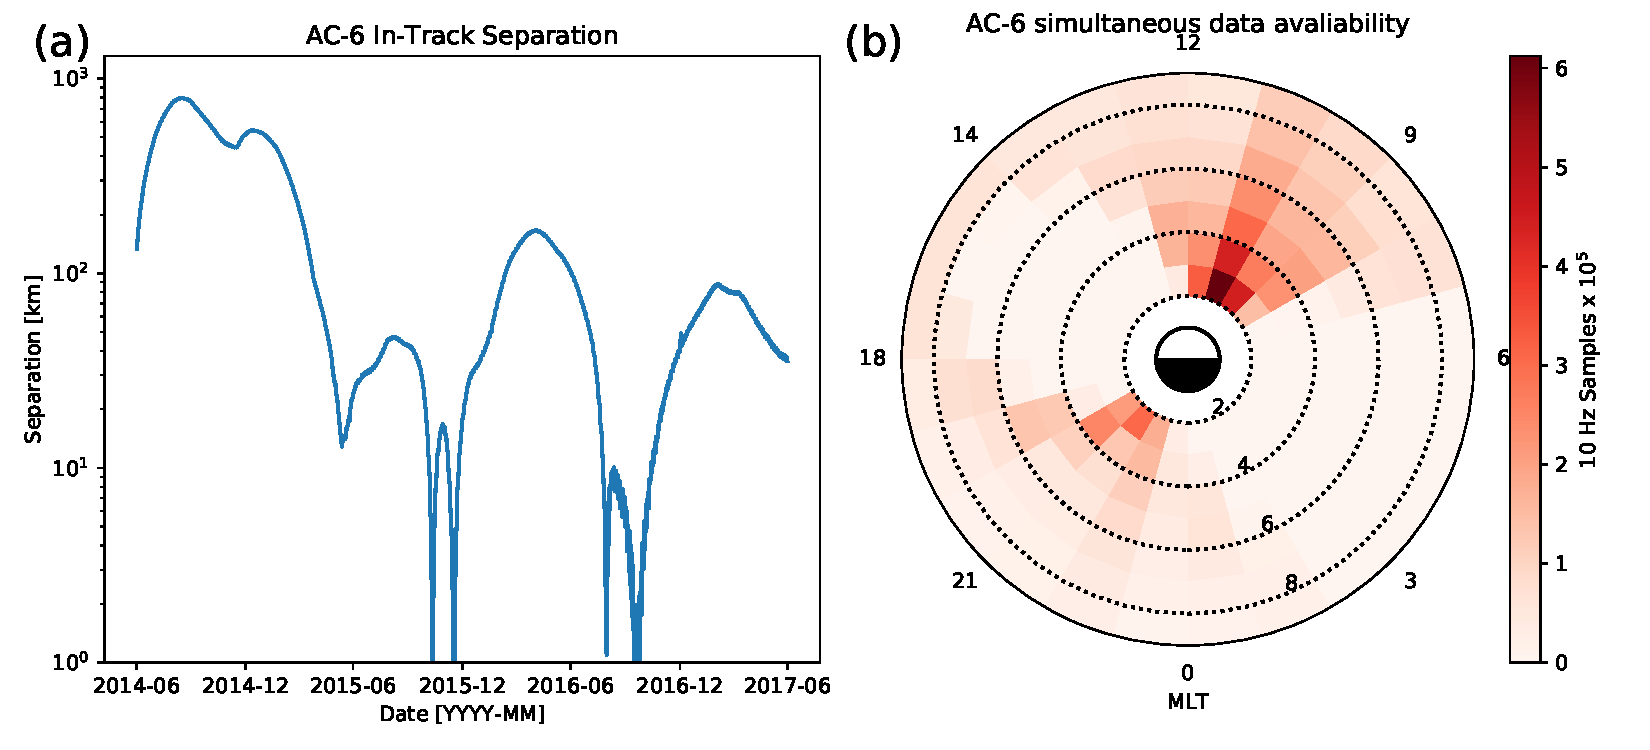
\includegraphics[width=\textwidth]{fig1.pdf}
\caption{AC6 mission distributions for (a) spacecraft separation and (b) number of simltaneous quality 10 Hz samples as a function of L and MLT.} \label{fig1}
\end{figure}

\section{Methodology} 
\subsection{Microburst Detection} \label{microburst_detection}
The first step to find microbursts observed simultaneously by AC6 is to identify them on each spacecraft separately. Microbursts were detected with two different methods that yielded quantitatively similar results. The first method is the burst parameter \cite{O'Brien2003}. This algorithm has been successfully used in other microburst studies, mainly with the microbursts observed by SAMPEX \textcolor{red}{add citations}. For AC6, a burst parameter threshold of 5 has good trade-off between false positive and false negative microburst detections. Another microburst detection algorithm based on wavelet spectra frequency filtering was developed and the resulting list of microbursts is similar to the list from the burst parameter.

Data cleaning to remove microburst-like transmitter noise was essential to this study. The transmitters on AC6 can cause unphysical count impulses in the dosimeters that resembles periodic trains of microbursts. One source of transmitter noise was observed at times when AC6 was in contact with the ground stations above the US for data downloads and commanding, thus the microburst detections made above the US that were mostly at low L were discarded. 

Another source of noise is crosslink transmissions between AC6-A and AC6-B. These transmissions occurred when either spacecraft transitioned from the survey mode to 10 Hz mode. This noise is sometimes not caught by the data quality flag, so the following empirically-derived criteria were developed to remove those detections. The dosimeter with a 250 keV nominal electron threshold, dos2, was used because it had a similar response to noise while rarely responded to microbursts. Since the transmitter noise is very periodic with a $\approx 0.2$ s period, cross-correlation (CC) and autocorrelation (AC) methods were applied to the dos1 and dos2 time series. Detections were removed if the following two criteria were met: either dos1 or dos2 time series had a AC peak at a $0.2$ or $0.4$ s lag and the dos1-dos2 CC was greater than 0.9. The AC lag criteria alone sometimes falsely removed legitimate trains of microbursts, so the second criteria insured that the detection was removed if there was an unphysically high correlation across an order of magnitude in energy.

The lists of microbursts observed individually by AC6 were then merged into a list of temporally correlated microbursts, i.e. microbursts that were observed simultaneously by both AC6 units, with the following procedure. The general idea is that a microburst detected by one spacecraft will cross-correlate well with the time series from the other spacecraft if it observed a similar microburst, and poorly if there was no microburst observed by the other spacecraft. Each microburst detection made by either spacecraft was cross-correlated with the time series from the other spacecraft. Windows with 1 and 1.2 s widths were used to CC the time series. Slightly different window sizes were used to account for random count variation due to Poisson noise. Microbursts detections that had a cross-correlation greater than $0.8$ were considered temporally coincident. This CC threshold was chosen as it is low enough to flag user-identified temporally coincident microbursts superposed with noise, and high enough to reject most non-coincident events. Figure \ref{fig2}, panels (a), (c), and (e) show examples of microbursts observed by both AC6 units when they were separated by 6, 17, and 69 km, respectively. 

The last CC criteria requires that the temporal CC must be greater than the spatial CC + 0.3. The spatial CC was calculated by shifting the AC6-B time series by the in-track lag to CC in the same spatial location, i.e. latitude. This criteria was applied to remove curtains, stationary structures observed by AC6 that are narrow in latitude \cite{Blake2016} that can be confused with microbursts. Figure \ref{fig2}, panels (b), (d), and (f) show the shifted time series to confirm that there were no spatially correlated, non-microburst structures present. Lastly the merged microburst list was spot checked by two authors to remove poorly correlated events. After filtering out transmitter noise and applying the CC criteria 662 simultaneous microburst detections were found and used for the analysis in the following section

\begin{figure}
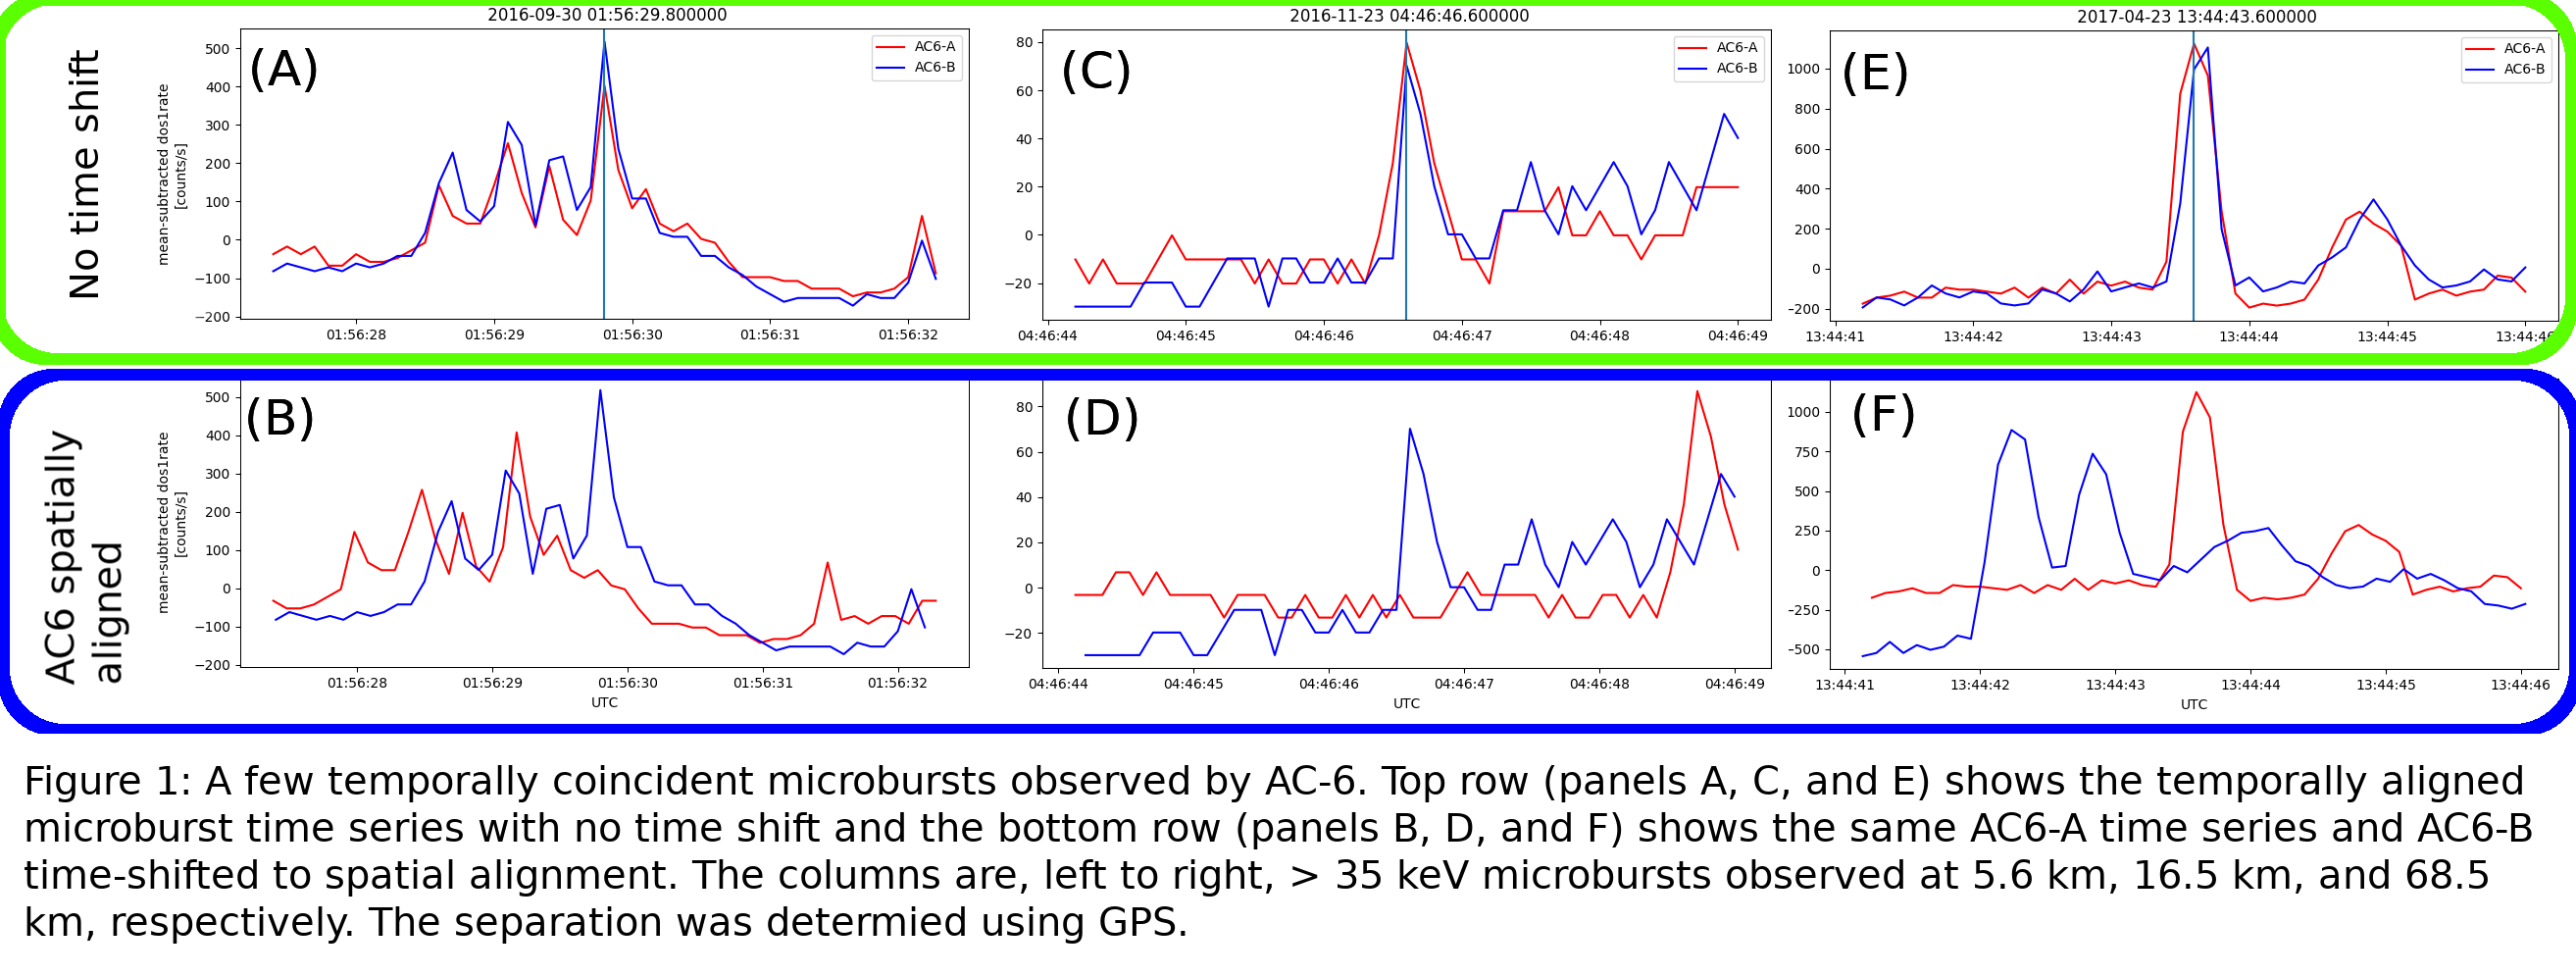
\includegraphics[width=\textwidth]{fig2.png}
\caption{Examples of microbursts observed simultaneously by AC6. Panels (a), (c) and (e) shows the temporally-aligned time series at spacecraft separations of 5.6 km, 16.5 km, and 68.5 km, respectively. Panels (b), (d), and (f) show the spatially aligned time series corresponding to the time series in the same column. The clear temporal correlation and lack of spatial correlation demonstrates that these events are microbursts. \textcolor{red}{I know not everyone has a microscope on their computer, and I plan to clean up this plot.}} 
\label{fig2}
\end{figure}
	

\subsection{Microburst Size Distribution in LEO and Magnetic Equator}\label{microburst_distribution}
The temporally coincident microbursts, which from now on will be referred to as microbursts, are now used to estimate the fraction of microbursts observed above AC6 separation, $s$. When AC6 observes a microburst at $s$, the microburst's size must be greater than $s$. This fact, along with the arguments presented in Section 4 in \citeA{Joy2002} who studied the most probable Jovian magnetopause and bow shock stand off distances, are used to investigate the dependence of the number of microbursts observed above $s$, as a function of $s$. This dependence is the microburst complementary cumulative distribution $\bar{F}(s)$. 

The cumulative number of microbursts observed above $s$ is the ratio of $N(s)$, the normalized number of microbursts observed above $s$, to $N(0)$, the total number of microbursts observed 
\begin{equation}
\bar{F}(s) = \frac{N(s)}{N(0)}.
\end{equation} The N(s) normalization attempts to account for AC6's uneven sampling as a function of $s$ and is defined by

\begin{equation}
N(s) = \sum_{i = s}^\infty n_{i} \frac{S_{max}}{S_{i}}
\end{equation} where $n_{i}$ is the number of microbursts observed by AC6 in ith separation bin. The normalization term $S_{max}/S_{i}$ is a ratio of the number of samples observed in the most sampled separation bin to the number of samples in the ith bin. This normalization factor corrects AC6's non-uniform sampling in separation by using the number of samples shown in Fig. \ref{fig3}c. With this normalization, $\bar{F}(s)$ can be interpreted as the fraction of microbursts observed above $s$ assuming AC6 sampled evenly in separation. Microburst $\bar{F}(s)$ in LEO is shown by the black curve in Fig. \ref{fig3}a for $4 < \mathrm{L}< 8$ and split into one L-wide bins with the colored curves. The separation bin width used in Fig. \ref{fig3} is 5 km. To check for bias in $\bar{F}(s)(s)$ due to the separation bins, $\bar{F}(s)(s)$ was resampled using other bin widths and offsets. Bin widths as large as $20-30$ km and bin offsets did not qualitatively effect the curves in Fig. \ref{fig3}a.

The overall trend in Fig. \ref{fig3}a consists of a sudden cumulative probability drop off, followed by a shoulder up to $s \approx 70$ km where $\bar{F}(s)$ drops to nearly zero. A large negative gradient of $\bar{F}(s)$ at a AC6 separation implies that microbursts must be smaller than that separation. To identify these separations, Fig. \ref{fig3}b shows the microburst probability density function (PDF), calculated by differentiating $\bar{F}(s)$. The microburst PDF shows a peak at $s < 30$ km as well as a peak between $70-80$ km separation. These PDF peaks are evidence of a sub $30$ km microburst population and larger microbursts observed up $70-80$ km separations. The shaded region around the black curves in Fig. \ref{fig3}a-b shows the standard error due to counting statistics. The uncertainty due to false coincidence events i.e. two unrelated microbursts lining up in time by random chance was also considered. The microburst duty cycle in a one minute window ($\approx 1 \ L$) around each microburst was calculated. The false coincidence probability is the square of the duty cycle and was found to be less than 5\% for the majority of microbursts. The false coincidence probability for each microburst was then used to randomly remove microbursts and $\bar{F}(s)$ was recalculated in $10^4$ trials. The spread in the $\bar{F}(s)$ trials with microbursts randomly removed was much smaller than the uncertainty due to counting statistics alone.

To compare the microburst size to the size of their progenitor waves, the spacecraft locations during observed microbursts were mapped to the magnetic equator using the Olson-Pfitzer magnetic field model \cite{Olson1982} which is implemented with a Python wrapper for IRBEM-Lib \cite{irbem}. As previously stated, a microburst observed in LEO has a size larger than the spacecraft separation, hence that microburst would also have a size larger than the spacecraft separation after it was mapped to the magnetic equator. Thus the procedure to estimate $\bar{F}(s)$ is identical to the LEO size distribution but with a different normalization. The normalization factors were calculated by mapping every quality AC6 sample to the magnetic equator and binning them by equatorial separation into 100 km wide bins. Figure \ref{fig4} shows the equatorial microburst size distribution in the same format as Fig. \ref{fig3}. The equatorial PDF trend is similar to LEO and most of the microbursts were observed when the AC6 equatorial separation was less than 300 km. 

The results in Figs. \ref{fig3} and \ref{fig4} show the fraction of microbursts observed above a spacecraft separation and do not fully represent the microbursts size distribution due to the compounding effects from the range of microburst sizes and random locations of microbursts with respect to AC6 i.e. even if the microburst size is much larger than $s$, some fraction of those microbursts will graze only one AC6 unit and not be observed by the other. Thus modeling is necessary to capture the compounding influence of these statistical effects on AC6.

\begin{figure}
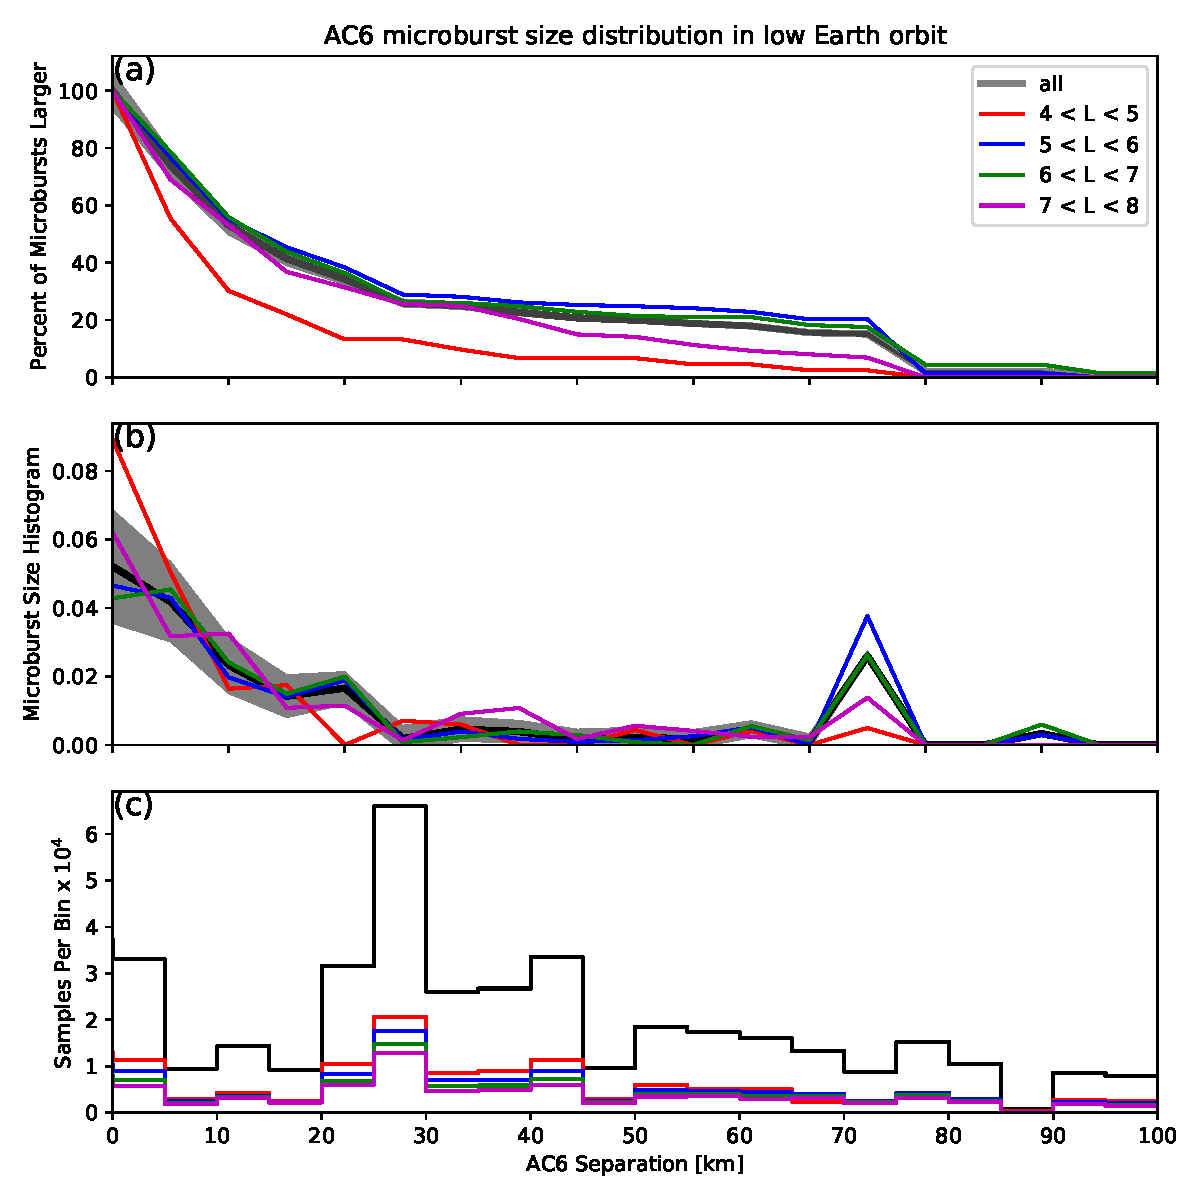
\includegraphics[width=\textwidth]{fig3.pdf}
\caption{Microburst size distribution in low Earth orbit. Panel (a) shows the percent of microbursts observed above that separation after accounting for the uneven separation sampling. Panel (b) shows the microburst probability density (size histogram) as a function of separation. Lastly, panel (c) shows the number of simultaneous samples AC6 observed as a function of separation. The colored lines show the distributions binned by L, and the thick black curve for the entire radiation belt ($4 < L < 8$). The gray shading around the black curve shows the uncertainty due to counting statistics.}
\label{fig3}
\end{figure}

\begin{figure}
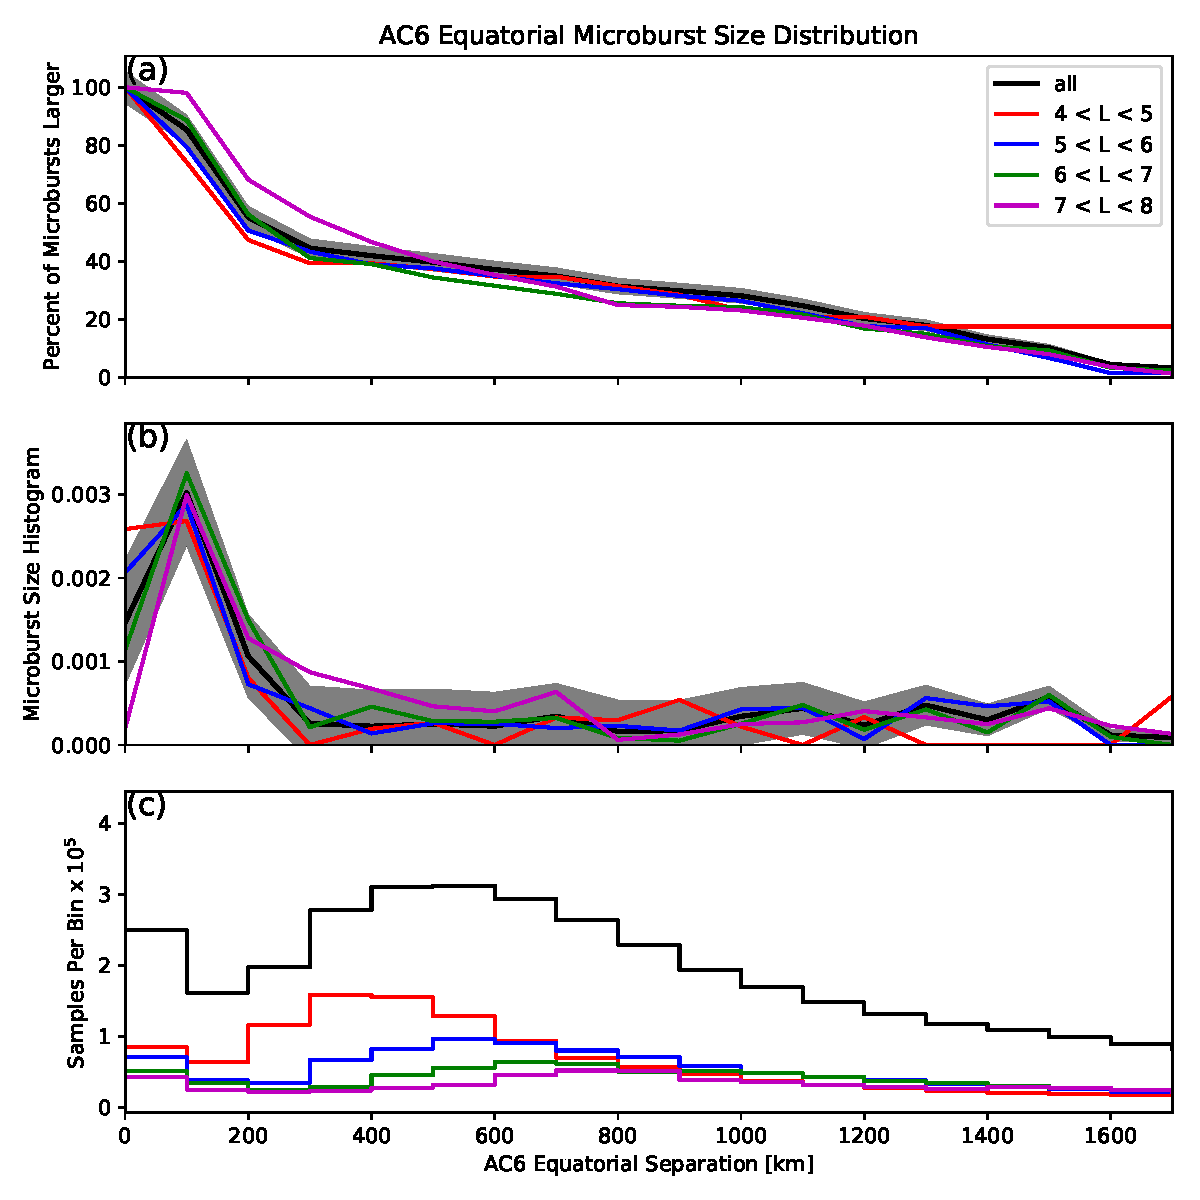
\includegraphics[width=\textwidth]{fig4.pdf}
\caption{Microburst size distribution mapped to the magnetic equator in the same format as Fig. \ref{fig3}.} 
\label{fig4}
\end{figure}

\section{Modeling the Distribution of Microburst Sizes} \label{model_section}
\subsection{Monte Carlo and Analytic Models to Estimate $\bar{F}(s)$}
To account for the effects due to microbursts randomly occurring in the vicinity of AC6 with an unknown distribution of microburst sizes, Monte Carlo (MC) and analytic models were developed. These models assume a hypothesized distribution of microburst sizes expressed with a probability density function $p(r)$, and a microburst footprint shape to estimate $\bar{F}(s)$. The microburst footprint is assumed to be circular with a radius $r$. Various microburst size distribution hypotheses were considered: a one-size microburst population, a two-size microburst population, and continuous $p(r)$ such as Maxwell, Weibull, and log-Normal.

The Monte Carlo model is the most intuitive and it consists of randomly scattering $10^5$ microburst centers in a 400 x 400 km grid around AC6 with random $r$ distributed according to a hypothesized $p(r)$. Spacecraft A is placed at the origin, and spacecraft B is placed along the positive y-axis at distances from spacecraft A corresponding to the AC6 separation bins used in Section \ref{microburst_distribution}. Then for each spacecraft B location, the number of circular microbursts that encompass both spacecraft was counted. The modeled fraction of microbursts observed above $s$ is then
\begin{equation}
\bar{F}(s) = \frac{\displaystyle\sum_{i > s}^\infty n_{i} }{ \displaystyle\sum_{i > 0}^\infty n_{i} }.
\end{equation} where as before the number of microbursts observed by both spacecraft in the ith bin is $n_{i}$.

The analytic model, while identical to the MC model, highlights the geometrical concepts connecting $p(r)$ and $\bar{F}(s)$. For a microburst with a diameter $d \geq s$ there is an area between AC6 where that microburst will be observed by both spacecraft. Figure \ref{fig5}a-c shows the geometry with the two spacecraft indicated with black dots under varying relations between $r$ and $s$. All microbursts who's center lies inside the circular area of radius $r$ that surrounds the top spacecraft will be observed by the top spacecraft. Likewise the same argument applies to the bottom spacecraft. If it exists, the intersection of these two circular areas defines another area, $A(r, s)$ where a microburst will be observed by both spacecraft and is given by the circle-circle intersection area equation, 
\begin{equation}
A(r, s) = 2r^2 \cos^{-1}{\Big( \frac{s}{2r} \Big)} - \frac{s}{2} \sqrt{4r^2 - s^2}.
\end{equation} Example geometries where $A(r, s) > 0$ are shown in Fig. \ref{fig5}b and c.

Now we develop the analytic $\bar{F}(s)$ given $p(r)$. For now we assume a one-sized $p(r)$ i.e., a delta function in $r$. Then the ratio of the circle intersection areas at two distinct AC6 separations $s_1$ and $s_2$ is the ratio of the number of microbursts observed at those two separations 

\begin{equation}
\frac{n_1}{n_2} = \frac{A(r, s_1)}{A(r, s_2)}.
\end{equation} Similar to the MC model \textcolor{red}{Move derivation to SI}

Then the analytic $\bar{F}(s)$ represents how quickly the fraction of microbursts observed by AC6 decreases as a function of $s$. 


 Furthermore the hypothesized $p(r)$ is the relative occurrence of microbursts at various $r$ and is effectively a weighting factor on $A(r, s)$ which must integrated out (marginalized) since AC6 is observing the cumulative effect of microbursts of all $r$. Lastly, a cumulative integral over a dummy variable $s'$ is applied to the normalized areas to calculate $\bar{F}(s)$. With these considerations the analytic $\bar{F}(s)$ is given by

\begin{equation} \label{analytic_integral}
\bar{F}(s) = \frac{\displaystyle\int\displaylimits_{s}^{\infty} \displaystyle\int\displaylimits_0^{\infty} A(r, s') p(r) dr ds'}{\displaystyle\int\displaylimits_{0}^{\infty} \displaystyle\int\displaylimits_0^{\infty} A(r, s') p(r) dr ds'}
\end{equation} where as in the Monte Carlo model the denominator normalizes $\bar{F}(s)$ to unity. To illustrate the effects of random microburst locations around AC6, example analytic and Monte Carlo model $\bar{F}(s)$ assuming a fixed-size $d = 40$ km microburst population is shown in Fig. \ref{fig5}d with the dashed blue and red curves, respectively.

\begin{figure}
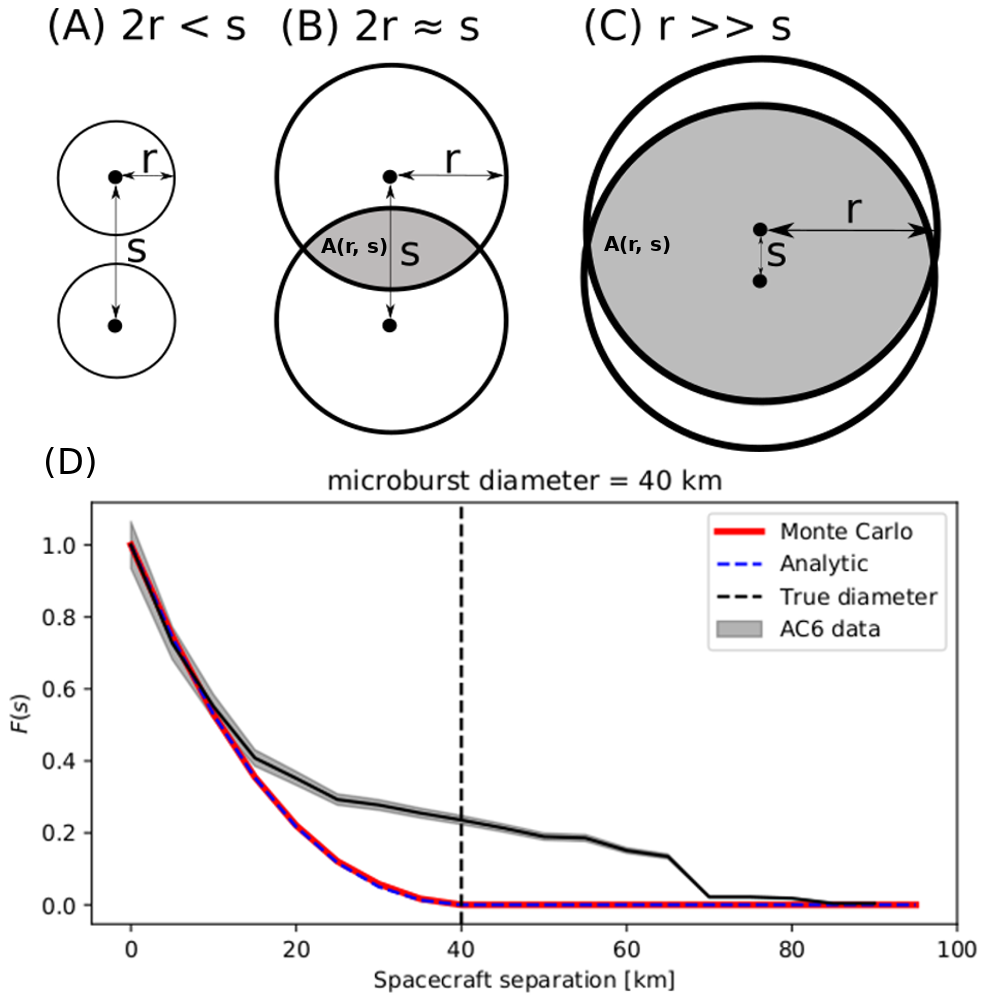
\includegraphics[width=\textwidth]{fig5.png}
\caption{Panels A-C show the varying geometries of the analytic model. The two spacecraft are shown as black dots. The enclosing black circle around each spacecraft bounds the area where a microburst will be observed by one or both AC6 units if the microburst's center lies somewhere inside the circle. Panel (A) shows the case where microburst diameter is smaller than the AC6 separation and all microbursts will be observed by either unit A or B and never simultaneously. Panel (B) shows the intermediate case where the microburst diameter is comparable to the AC6 separation and some fraction of microbursts will be observed simultaneously. The fraction of the microbursts simultaneously observed is proportional to the circle intersection area shown with grey shading. Panel (C) shows the case where the microburst diameter is much larger than the spacecraft separation and nearly all microbursts will be observed by both spacecraft. Lastly panel (D) shows $\bar{F}(s)$ from the AC6 data with a solid black line, and a MC and analytic $\bar{F}(s)$ curves for a single-sized microburst distribution with a 40 km diameter.} 
\label{fig5}
\end{figure}

\subsection{Estimating optimal parameters for microburst size models}
At this stage a few hypothesized $p(r)$ are tested and optimal model parameters estimated. For each hypothesized $p(r)$, Bayesian inference is used to estimate the optimal model parameters with a Metropolis Markov Chain Monte Carlo (MCMC) sampler \cite{Metropolis1953}. Bayes theorem is central to Bayesian inference. Given the observed $\bar{F}(s)$ designated here with $x$, and $p(r)$ model parameters with $\theta$, Bayes theorem can be written as

\begin{equation}
p(\theta | x) = \frac{p(x | \theta) p(\theta)}{p(x)}
\end{equation} where $p(\theta)$ is the prior probability distribution for each model parameter that describes the prior level of knowledge, however weak, about the model parameters. The likelihood is $p(x | \theta)$ that describes the probability of obtaining $x$ given the tested model parameters. The likelihood facilitates the MC (or analytic) microburst model to map from $\theta$ to $\bar{F}(s)$. The posterior distribution, $p(\theta | x)$ is the updated $\theta$ distribution given the observations and prior. The posterior is used here to make conclusions regarding the range of model parameters that are consistent with the observations after assuming a likelihood function and prior knowledge of the model parameters. Lastly, $p(x)$ is the marginal likelihood that describes the probability of obtaining $x$ after marginalizing over all prior variables. Calculation of $p(x)$ is difficult, and often not necessary for model parameter estimation. 

With all of the above terminology, the important takeaway is that the posterior distribution for each model parameter is interpreted as the range of $\theta$ consistent with $x$. A 95\% credible interval (CI) is reported here that is interpreted as: assuming a hypothesized $p(\theta, r)$, there is a 95\% probability that the true $\theta$ is inside the CI. To sample the posterior distribution, the $\theta$ parameter space is explored with the Metropolis sampler.

While the Metropolis sampler is explained in detail in \citeA{Metropolis1953} and a good introduction given in \citeA{Sambridge2006}, a brief overview is warranted. The Metropolis sampler samples the posterior distribution in $N$ trials. For each trial a random $\theta$ is chosen from the prior for which the posterior is estimated. After the initial $\theta$, the Metropolis MCMC chooses a new $\theta$ nearby in parameter space. If the prior probability of the new $\theta$ multiplied by the likelihood is higher the current $\theta$, the MCMC accepts the new $\theta$, otherwise there is a random chance that the new $\theta$ will be accepted or rejected. This accept/reject criteria allows the sampler to trend to more probable $\theta$ while also exploring the neighboring regions. After the $N$ trials, a histogram is made with the accepted $\theta$ to produce the posterior distribution for each model parameter.

A one-size microburst population model is explored first and the microburst PDF is given by 
\begin{equation}
p(d) = \delta(s-d)
\end{equation} where $\delta$ is the Dirac Delta function and $d$ is the diameter of all microbursts. The range of $d$ that is consistent with the observed $\bar{F}(s)$ is shown in Fig. \ref{fig6}. Assuming this model, there is a $95 \%$ probability that the microburst size is between 38 and 129 km with the optimal size of 73 km, estimated from minimizing the least squares penalty function. 

A generalization of the one-size model is a two-size microburst population model that assumes the following microburst PDF
\begin{equation}
p(d) = a \delta(s-d_0) + (1-a)\delta(s-d_1)
\end{equation} where the diameters of the two microburst populations is given by $d_0$ and $d_1$ and $a$ is the parameter that quantifies the relative fractions of the two populations. The result of this model is shown in Fig. \ref{fig7}. The fit is slightly better than the one-size model, although that is to be expected assuming two more free model parameters. A majority, $98$ \% of microbursts, have a size between $12$ and $47$ km with a rare population with a size between 76 and 234 km. The set of parameters that minimize least squares is $99.5$ \% of microbursts are small with a size of $21$ km and the $0.5$ \% of microbursts have a 140 km size.

\begin{figure}
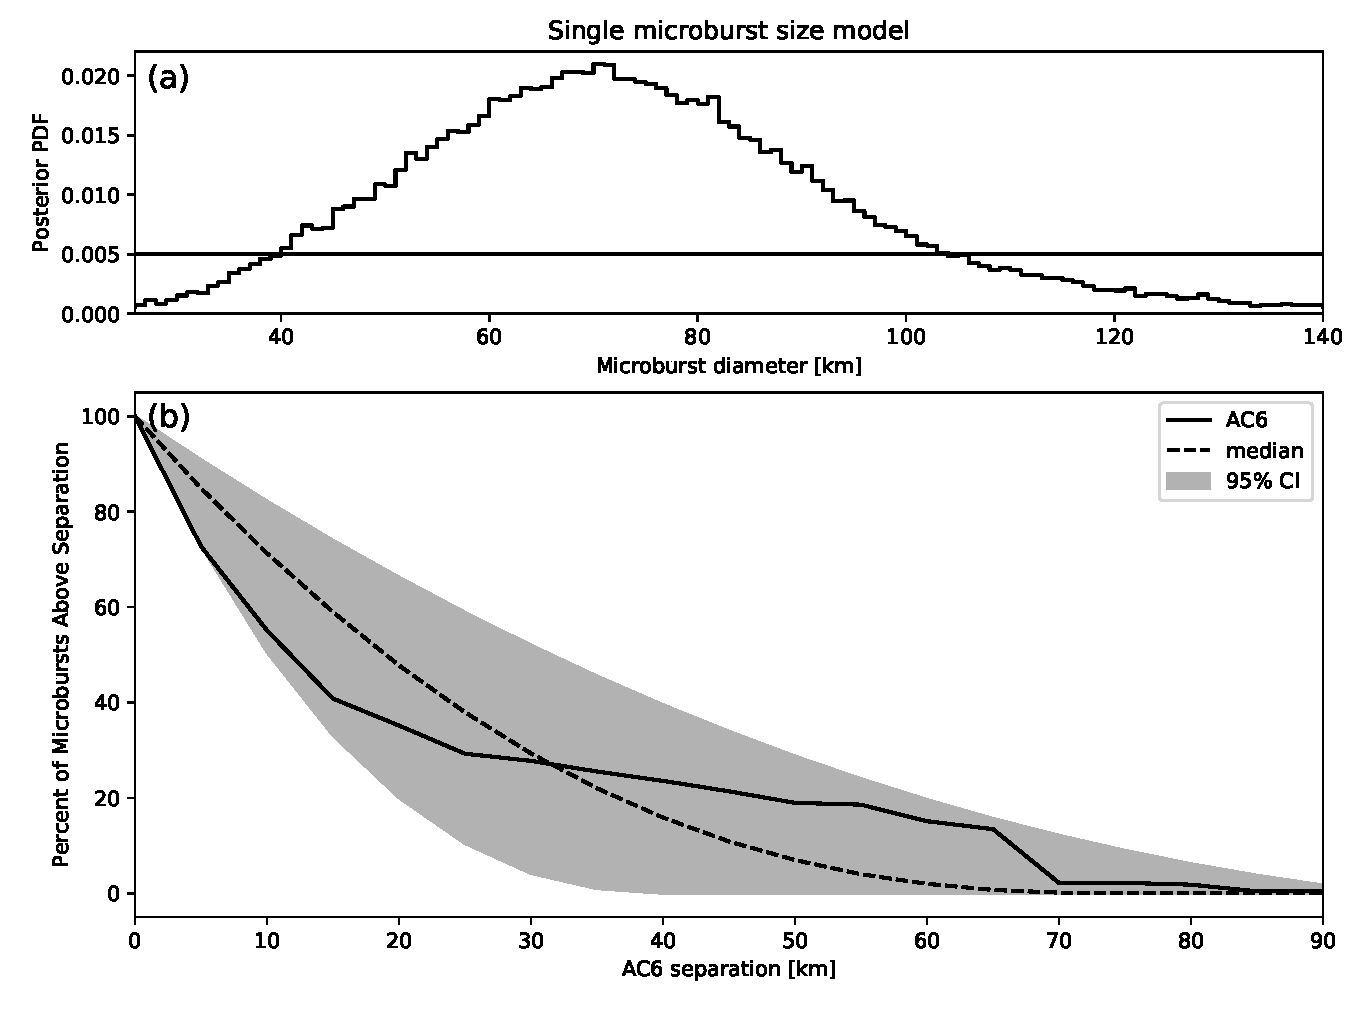
\includegraphics[width=\textwidth]{fig6.pdf}
\caption{Range of plausible microburst sizes assuming all microbursts are one fixed size. Panel (a) shows the posterior probability density function of microburst diameters in black. The red, green, and blue vertical lines at 38, 73, and 129 km represent the 2.5, 50, and 97.5 posterior percentiles, respectively. A uniform prior between 0 and 200 km was assumed for this MCMC run and is shown in cyan. Panel (b) shows the percent of microbursts observed above an AC6 separation for $4 < L < 8$ in black. The 2.5, 50 and 97.5 size percentiles were estimated from the posterior and plotted in red, green, and blue curves, respectively.} 
\label{fig6}
\end{figure}

\begin{figure}
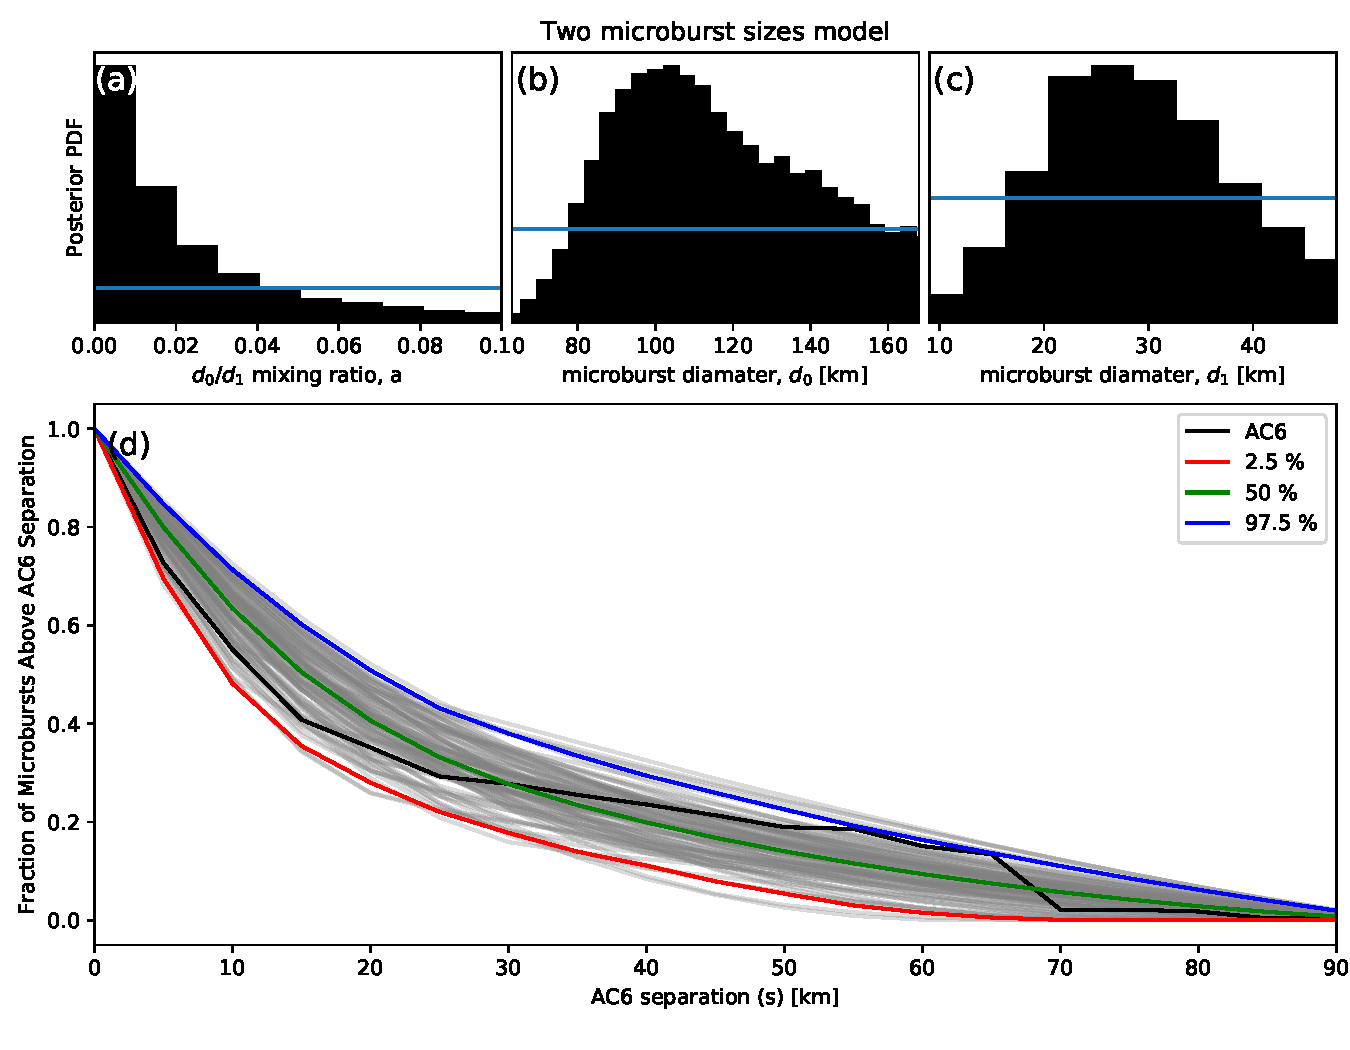
\includegraphics[width=\textwidth]{fig7.pdf}
\caption{Plausible microburst percent curves assuming microburst size distribution is bimodal consisting of two sizes $d_0$ and $d_1$ with a mixing term that quantifies the relative occurrence of the $d_0$ to $d_1$ microburst populations. Panel (a) shows the posterior distribution for the microburst population mixing term, $a$ with a median value of $0.02$. The $a$ prior was uniform between 0 and 0.2. Panel (b) shows the posterior distribution for $d_0$, the larger microburst population estimated with a uniform prior between 50 and 200 km and the posterior median diameter of $122$ km. Panel (c) shows the posterior distribution for $d_1$, the smaller microburst population, estimated using a uniform prior between 0 and 50 km with a median diameter of $28$ km. Panel (d) is similar to Fig. \ref{fig6}b and shows the AC6 microburst fraction for $4 < L < 8$ in black. A set of 1000 random parameter triples ($a$, $d_0$, and $d_1$) were drawn from the posterior and used to generate a family of $\bar{F}(s)$ curves. At each $s$ the range of consistent $\bar{F}(s)$ were quantified by the 2.5, 50 and 97.5 percentiles and shown with the red, green, and blue curves, respectively.} 
\label{fig7}
\end{figure}

\section{Discussion} \label{discussion}
The LEO microburst $\bar{F}(s)$ estimated in section \ref{microburst_distribution} shows that a majority of coincident microbursts were observed by AC6 when they were separated by less than a few tens of km. This conclusion is consistent with prior literature and most similar to \citeA{Parks1967} who reported that $> 15$ keV microbursts are $40 \pm 14$ km and the bouncing packet example shown in \citeA{Blake1996} with a size of ``at least a few tens of kilometers". The AC6 microburst size distribution is much larger than the sizes reported in \citeA{Dietrich2010} who used very low (VLF) frequency transmission paths and SAMPEX to conclude that microbursts must be smaller than 4 km from a small number of microbursts observed during one SAMPEX pass. \citeA{Dietrich2010} arrived at their conclusion by looking for temporal coincidence of microbursts and FAST events, subsecond VLF transmission perturbations, but the connection between FAST events and microbursts is not well understood. Lastly, our new results are consistent with FIREBIRD-II observations of a $> 11$ km microburst reported by \citeA{Crew2016}. The small number of microbursts observed by AC6 up to $s \approx 70$ km are consistent with the $> 51$ km bouncing packet microburst reported in \citeA{Shumko2018a}. 

The microburst PDF shown in Fig. \ref{fig3}b shows evidence of a bimodal microburst size distribution. The quality of the AC6 data is insufficient to definitively conclude that there are two distinct microburst populations. This has been suggested before by \citeA{Blake1996} who noted that the $> 150$ keV and $> 1$ MeV microbursts are not always well correlated e.g. Fig. 10 in \citeA{Blake1996}. The different microburst population hypothesis can be better tested with an AC6-like mission with better energy resolution and homogeneous MLT coverage.

The model results from section \ref{model_section} emphasize that care must be taken to compare the $\bar{F}(s)$ curves observed by AC6 and the true microburst size distribution due to the compounding effect of an unknown microburst size distribution, unknown microburst shape, and random microburst locations near AC6. By naively assuming there is only one microburst size, the results in Fig. \ref{fig6} suggest that there is a 95\% probability that the microburst size is somewhere between 38 and 129 km, a relatively wide range of values. The two-size model microburst from Fig. \ref{fig7} has a smaller variance around the AC6 $\bar{F}(s)$, which is expected with the addition of two more free parameters. The two size model is interpreted as 98\% of microbursts sizes are between 12 and 47 km and larger microbursts are very uncommon. A variety of continuous $p(r)$ such as the Maxwellian, Weibull and log-normal were also tested with similar results and are not shown. While the two-size model quantitatively fits the observations the best out of all $p(r)$ tested, nature surely does not only have two microburst sizes. Rather the most realistic PDF hypothesis would be bimodal and continuous. Due to lack of prior observations and theoretical predictions, it is difficult to identify a more appropriate $p(r)$ hypothesis at this time.

The equatorial microburst $\bar{F}(s)$ estimated in section \ref{microburst_distribution} can be compared to prior multi-point measurements of chorus source sizes made near the magnetic equator. The International Sun-Earth Explorers (ISEE 1 and 2) were used by \citeA{Gurnett1979} to make one of the first direct chorus source scale measurements. \citeA{Gurnett1979} estimated that the wave power correlation scale was on the order of a few hundred km across the background magnetic field. Using the Cluster Wide Band Data measurements \citeA{Santolik2003} found the correlation scale of whistler mode chorus waves to be around 100 km near the source region at $L \approx 4$ and midnight MLT sector. Furthermore, \citeA{Turner2017} used the four satellites comprising the Magnetospheric Multiscale Mission and found that rising tone whistler mode chorus elements were phase coherent up to 70 km at $L \approx 8$. Lastly, \citeA{Agapitov2010, Agapitov2011b, Agapitov2017a, Agapitov2018} used multiple sets of spacecraft missions with wave measurements near the chorus source region to statistically show that the extent of chorus source region can extend from 600 km in the outer radiation belt to greater than 1,000 km in the outer magnetosphere. 

With the prior chorus wave size estimates and microburst probability density from Fig. \ref{fig4}b in mind, it appears that the majority of microbursts were observed when the equatorial AC6 separation was less than $200$ km. Assuming that chorus waves scatter electrons as in prior literature \cite<e.g.,>[]{Lorentzen2001a, Breneman2017}, then the chorus waves that scatter microburst electrons on those scales must have correlated properties on those scales. The wave properties necessary for scattering microburst electrons e.g. coherence, polarization, wave normal angle, can be identified by studying the waves properties that are only observed by multiple equatorial spacecraft at small separations. These properties can then aid wave-particle scattering model development by constraining the wave properties and scattering modes responsible for scattering microburst electrons. These models may then be capable of predicting the distribution of microburst sizes that should be observed in LEO.

\section{Conclusions}
In conclusion, the twin AC6 CubeSats enabled the detailed statistical study of microburst sizes from a two point measurement platform. Roughly $60 \%$ of the $> 30$ keV microbursts were simultaneously observed while AC6 was separated by less than $20$ km and the rest were observed up to $\approx 80$ km separation. The microburst cumulative distribution function is essential to model and quantify the relationship between the number of microbursts observed as a function of separation to a hypothesized microburst size distributions. The AC6 microburst data together with modeling, has hinted at the existence of a bimodal microburst size PDF with the majority of microbursts smaller than $40$ km, and a rare microburst population with a size around $100$ km. The bimodal size hypothesis may be more comprehensively addressed from LEO spacecraft with more microburst observations for spacecraft separations up to $100$ km, homogeneous MLT coverage, and differential energy channels. Moreover, to disentangle the compounding effect that affects two-point microburst measurements, a X-ray imager on a high altitude balloon can observe the atmospheric microburst footprint and determine the microburst size, shape, and any spatial correlations without ambiguity. 

When mapped to the magnetic equator, most microbursts were observed while the mapped AC6 separation was less than $200$ km. This correlates well with the sizes of highly correlated chorus waves and it suggests that the wave properties crucial for scattering microbursts must be correlated on relatively small regions. By studying the wave properties that are correlated on a few hundred km scales, the dominant wave scattering modes may be identified.


%%%%%%%%%%%%%%%%%%%%%%%%%%%%%%%%%%%%%%%%%%%%%%%%%%%%%%%%%%%%%%%%
%
%  ACKNOWLEDGMENTS
%
% The acknowledgments must list:
%
% >>>>	A statement that indicates to the reader where the data
% 	supporting the conclusions can be obtained (for example, in the
% 	references, tables, supporting information, and other databases).
%
% 	All funding sources related to this work from all authors
%
% 	Any real or perceived financial conflicts of interests for any
%	author
%
% 	Other affiliations for any author that may be perceived as
% 	having a conflict of interest with respect to the results of this
% 	paper.
%
%
% It is also the appropriate place to thank colleagues and other contributors.
% AGU does not normally allow dedications.


\acknowledgments
This work was made possible with the help from the many engineers and scientists at the Aerospace Corporation who successfully designed, built, and operated AC6. M. Shumko was supported by NASA Headquarters under the NASA Earth and Space Science Fellowship Program - Grant 80NSSC18K1204. \textcolor{red}{Other Aerospace and MSU funding sources...} The AC6 data is available at http://rbspgway.jhuapl.edu/ac6 and the IRBEM-Lib version used for this analysis can be downloaded from https://sourceforge.net/p/irbem/code/616/tree/.

%% ------------------------------------------------------------------------ %%
%% References and Citations

%%%%%%%%%%%%%%%%%%%%%%%%%%%%%%%%%%%%%%%%%%%%%%%
%
% \bibliography{<name of your .bib file>} don't specify the file extension
%
% don't specify bibliographystyle
%%%%%%%%%%%%%%%%%%%%%%%%%%%%%%%%%%%%%%%%%%%%%%%

\bibliography{/home/mike/Dropbox/0_firebird_research/A_presentations/refs}

%Reference citation instructions and examples:
%
% Please use ONLY \cite and \citeA for reference citations.
% \cite for parenthetical references
% ...as shown in recent studies (Simpson et al., 2019)
% \citeA for in-text citations
% ...Simpson et al. (2019) have shown...
%
%
%...as shown by \citeA{jskilby}.
%...as shown by \citeA{lewin76}, \citeA{carson86}, \citeA{bartoldy02}, and \citeA{rinaldi03}.
%...has been shown \cite{jskilbye}.
%...has been shown \cite{lewin76,carson86,bartoldy02,rinaldi03}.
%...has been shown \cite [e.g.,][]{lewin76,carson86,bartoldy02,rinaldi03}.
%
% DO NOT use other cite commands (e.g., \citet, \citep, \citeyear, \nocite, \citealp, etc.).
%



\end{document}



More Information and Advice:

%% ------------------------------------------------------------------------ %%
%
%  SECTION HEADS
%
%% ------------------------------------------------------------------------ %%

% Capitalize the first letter of each word (except for
% prepositions, conjunctions, and articles that are
% three or fewer letters).

% AGU follows standard outline style; therefore, there cannot be a section 1 without
% a section 2, or a section 2.3.1 without a section 2.3.2.
% Please make sure your section numbers are balanced.
% ---------------
% Level 1 head
%
% Use the \section{} command to identify level 1 heads;
% type the appropriate head wording between the curly
% brackets, as shown below.
%
%An example:
%\section{Level 1 Head: Introduction}
%
% ---------------
% Level 2 head
%
% Use the \subsection{} command to identify level 2 heads.
%An example:
%\subsection{Level 2 Head}
%
% ---------------
% Level 3 head
%
% Use the \subsubsection{} command to identify level 3 heads
%An example:
%\subsubsection{Level 3 Head}
%
%---------------
% Level 4 head
%
% Use the \subsubsubsection{} command to identify level 3 heads
% An example:
%\subsubsubsection{Level 4 Head} An example.
%
%% ------------------------------------------------------------------------ %%
%
%  IN-TEXT LISTS
%
%% ------------------------------------------------------------------------ %%
%
% Do not use bulleted lists; enumerated lists are okay.
% \begin{enumerate}
% \item
% \item
% \item
% \end{enumerate}
%
%% ------------------------------------------------------------------------ %%
%
%  EQUATIONS
%
%% ------------------------------------------------------------------------ %%

% Single-line equations are centered.
% Equation arrays will appear left-aligned.

Math coded inside display math mode \[ ...\]
 will not be numbered, e.g.,:
 \[ x^2=y^2 + z^2\]

 Math coded inside \begin{equation} and \end{equation} will
 be automatically numbered, e.g.,:
 \begin{equation}
 x^2=y^2 + z^2
 \end{equation}


% To create multiline equations, use the
% \begin{eqnarray} and \end{eqnarray} environment
% as demonstrated below.
\begin{eqnarray}
  x_{1} & = & (x - x_{0}) \cos \Theta \nonumber \\
        && + (y - y_{0}) \sin \Theta  \nonumber \\
  y_{1} & = & -(x - x_{0}) \sin \Theta \nonumber \\
        && + (y - y_{0}) \cos \Theta.
\end{eqnarray}

%If you don't want an equation number, use the star form:
%\begin{eqnarray*}...\end{eqnarray*}

% Break each line at a sign of operation
% (+, -, etc.) if possible, with the sign of operation
% on the new line.

% Indent second and subsequent lines to align with
% the first character following the equal sign on the
% first line.

% Use an \hspace{} command to insert horizontal space
% into your equation if necessary. Place an appropriate
% unit of measure between the curly braces, e.g.
% \hspace{1in}; you may have to experiment to achieve
% the correct amount of space.


%% ------------------------------------------------------------------------ %%
%
%  EQUATION NUMBERING: COUNTER
%
%% ------------------------------------------------------------------------ %%

% You may change equation numbering by resetting
% the equation counter or by explicitly numbering
% an equation.

% To explicitly number an equation, type \eqnum{}
% (with the desired number between the brackets)
% after the \begin{equation} or \begin{eqnarray}
% command.  The \eqnum{} command will affect only
% the equation it appears with; LaTeX will number
% any equations appearing later in the manuscript
% according to the equation counter.
%

% If you have a multiline equation that needs only
% one equation number, use a \nonumber command in
% front of the double backslashes (\\) as shown in
% the multiline equation above.

% If you are using line numbers, remember to surround
% equations with \begin{linenomath*}...\end{linenomath*}

%  To add line numbers to lines in equations:
%  \begin{linenomath*}
%  \begin{equation}
%  \end{equation}
%  \end{linenomath*}



